\documentclass[10pt]{jsarticle}
\usepackage{gaiyou}
\usepackage[dvipdfmx]{graphicx}
\usepackage[top=2cm, bottom=2cm, left=1.5cm, right=1.5cm]{geometry}

\begin{document}

\pagestyle{empty}

\setlength{\baselineskip}{13truept}

\title{植物自律化による自己育成システム}
\engtitle{Self-cultivation system by plant autonomization}
\supervisor{村松 聡}
\author{黒木 駿太}
\engsupervisor{Satoshi Muramatsu}
\engauthor{Shunta Kuroki}

\maketitle
\thispagestyle{empty}

\section{はじめに}
近年、植物の栽培方法は多様化しハウス栽培や水耕栽培に留まらず、屋内の植物工場で栽培される事例もある。
植物工場ではコンピュータ制御による管理が行われていることがあり、水分や肥料といった物質の管理や、光や温湿度といった環境までも栽培されている植物に最適化されるようプログラムされている。
しかし、工場で作物を栽培するためにはめに建設の資金と時間を必要とすることや、栽培する植物は水耕栽培で採算性の良い品種の植物に限られてしまうことがある。
また、最終的には人間が管理を行わければならない問題がある。

その一方、人間を始めとする動物は自発的に飲食や移動をを行い、自らの生命は他者に依存することなく最適な環境を獲得する。これらの特徴は動物のメリットである。
このことから、植物も動物のような能動的に生命の欲求を満たすことで、他者の助けなしに最適な環境を見つけ出し、効率的に生命活動を行うことが可能となる。

そこで本研究は人間による管理を必要としない、植物の能動的な行動で自己成長が行えるシステムの開発を行う。

\section{植物自律化}
植物自律化とは、能動的に行動を行う植物を意味し。
具体的にはセンサにより自己状態を把握し、必要に応じてロボットで移動することを指す。
土壌の水分が減ると水分補給を行い、日差しが弱い場合にはより明るい場所を探すよう能動的に行動を行う事が可能となる。
それにより、動物のように自身の状態によって自由に行動し、他者に依存することのない自律化を実現する。

\section{自動育成植木鉢ロボットシステム}
前章の植物自律化を行うために自動育成植木鉢ロボットシステムの製作を行った。
本システムではセンサ情報を元に作成された地図を用いてロボットの行動計画を行う。
地図情報は移動を行うごとに随時追加され、時間とともに情報の信頼性と予測精度が向上する。
Fig.\ref{robot_all}の本システムでは植物と環境センサを搭載し走行する自律移動ロボットと、水分を供給する給水ステーションにわかれている。
\begin{figure}[ht]
    \centering
    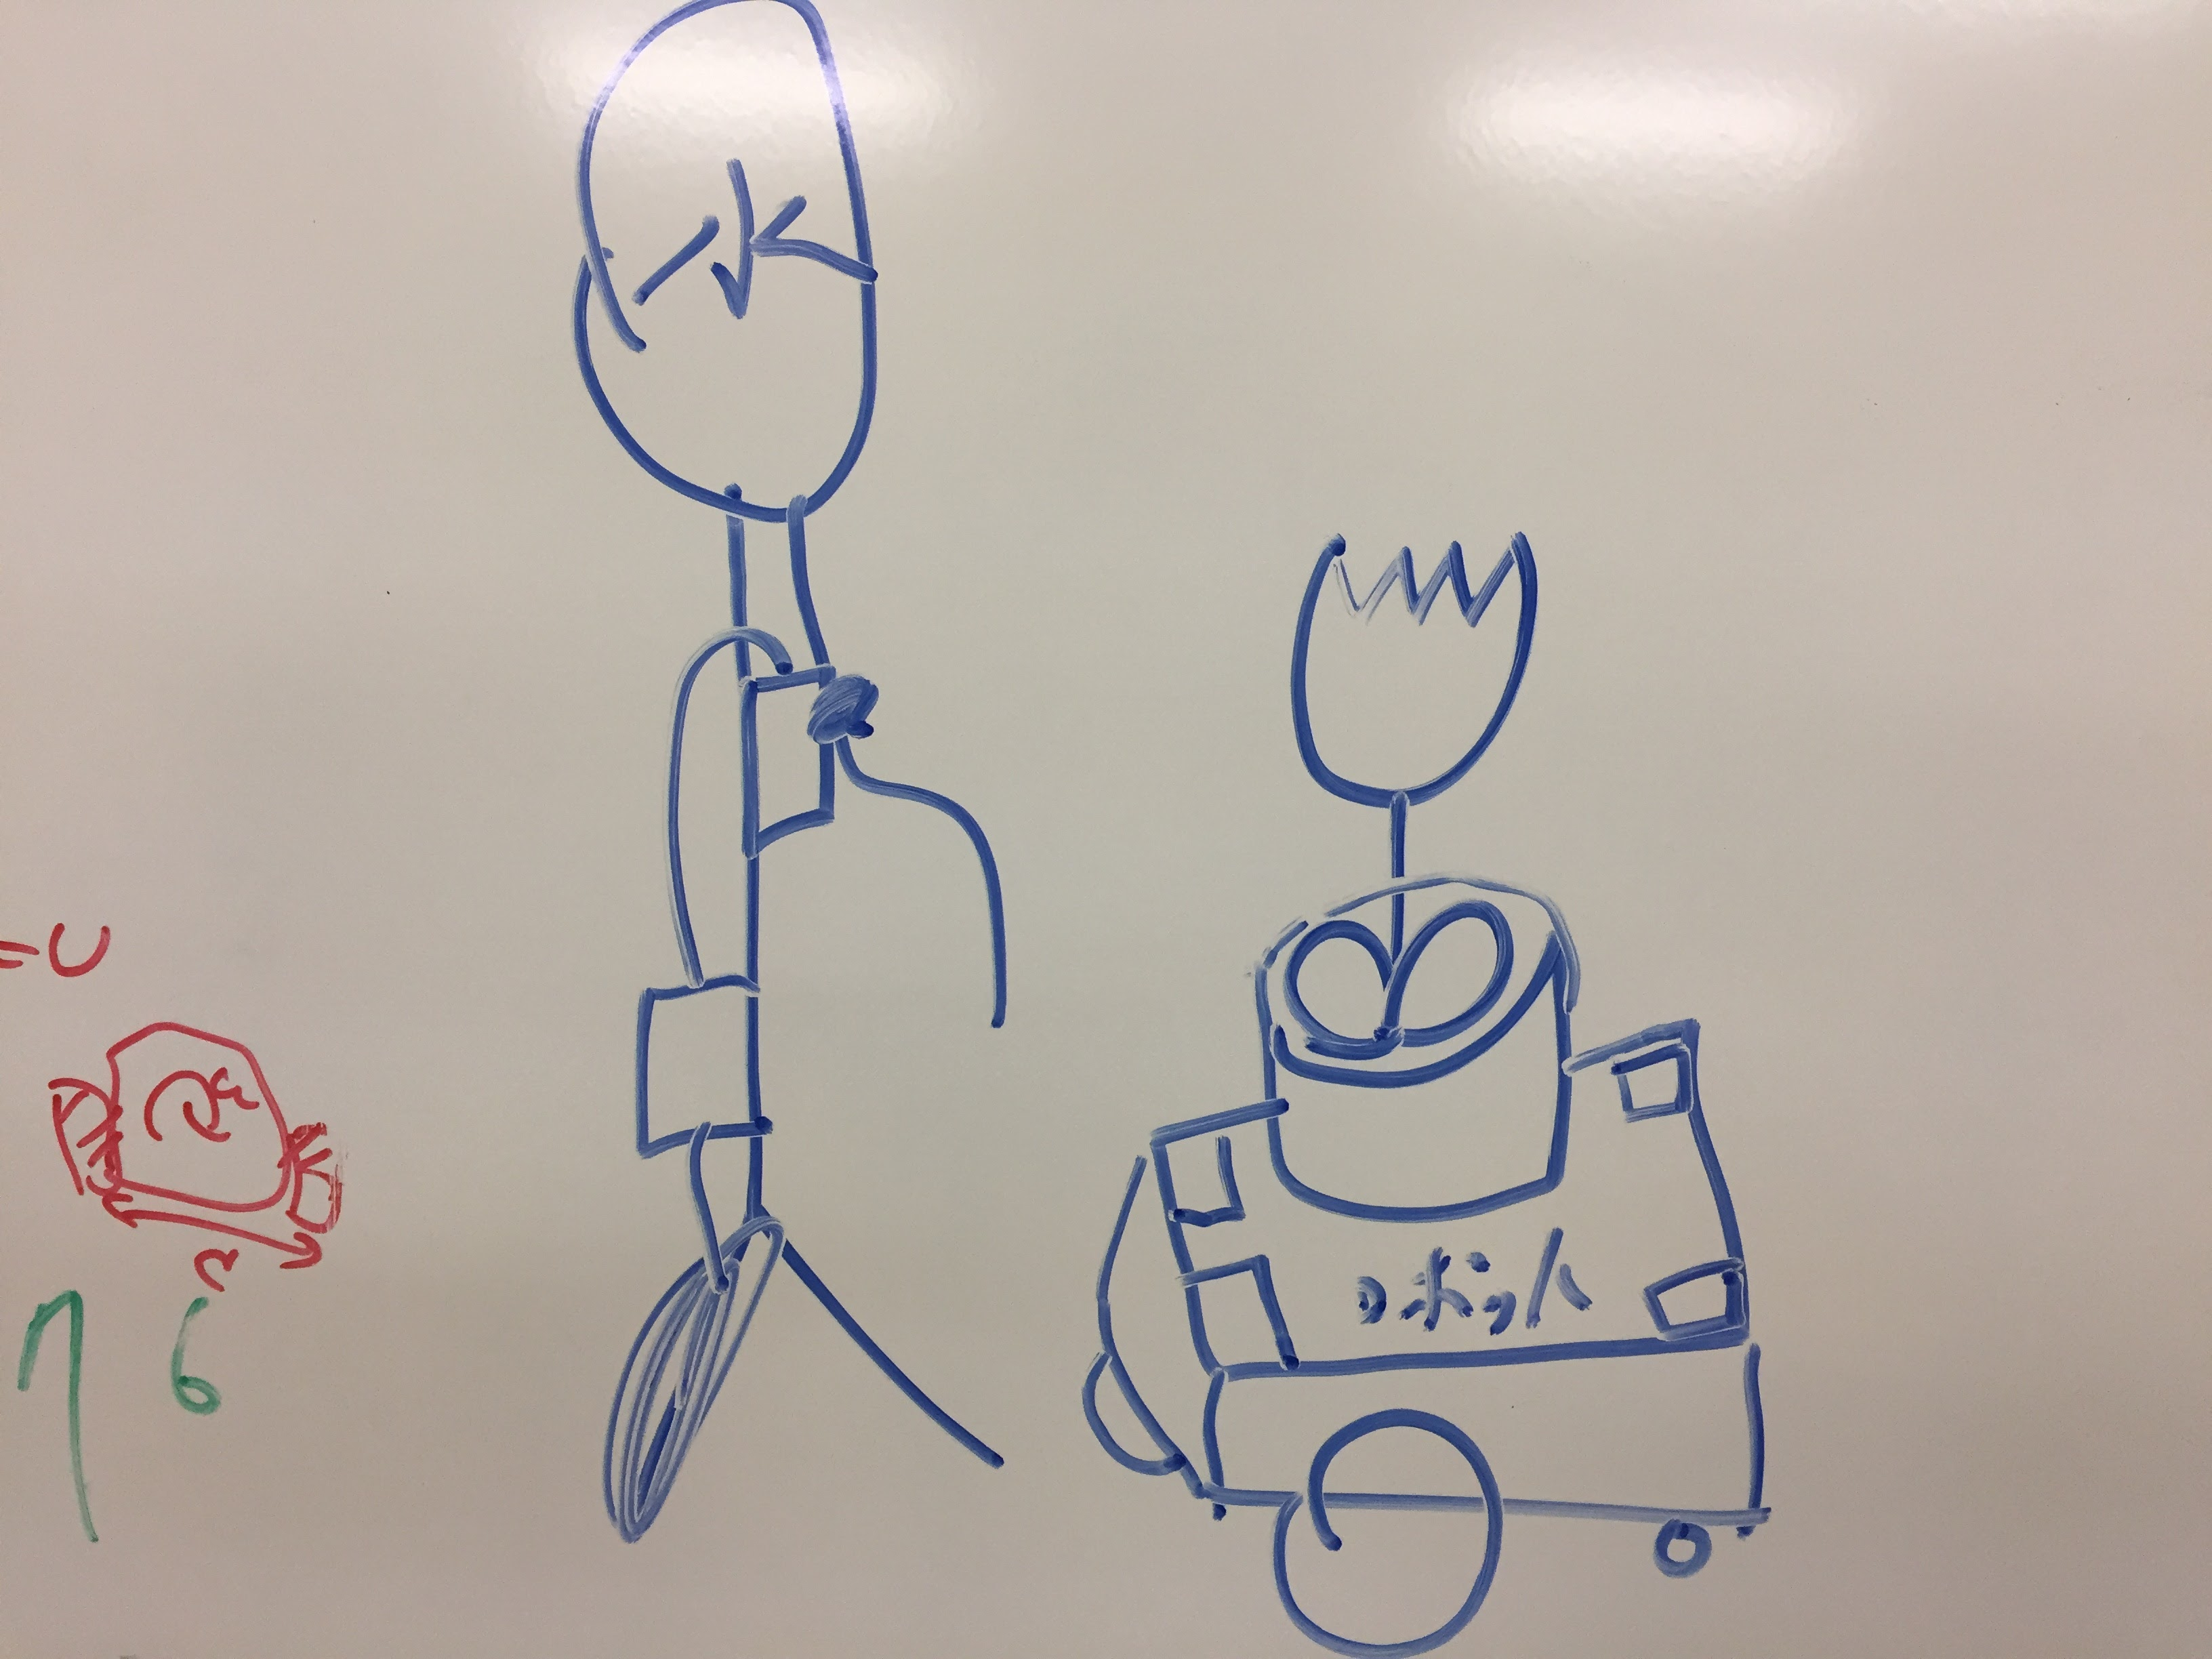
\includegraphics[width=0.4\textwidth]{img/IMG_3894.JPG}
    \caption{ロボットシステム全体}
    \label{robot_all}
\end{figure}
\subsection{自律移動ロボット}
自律移動を行うためには植木鉢の搭載が可能な移動機構が必須となる。
走行中でも植木鉢が安定し、狭い場所においても旋回が可能なものであり、比較的消費電力の少ないロボットが対象となる。
以上の条件より、製作コストも少ない対向2輪型ロボットを用いた自律移動ロボットの製作を行った。
路面との接地面が3点でグラつきがなく、制御も比較的行い易い。
また、環境情報を取得するセンサ類を搭載することで自律移動の手助けを行っている。
ロボットの制御には小型コンピュータを中心としたものになっており、ネットワークを介することで他の機器とも連携が容易となっている。
\subsubsection{ハードウェア}
ロボットの筐体は安全性と管理の観点から2段に分かれておいる。下段にはモータや制御機器などの電装系、上段にはセンサ類と植木鉢を設置し、サイドカバーをつけることで水濡れによるショートやデザイン性の向上を図っている。
ロボット構成はFig.\ref{robot_hard}のようになっている。
\begin{figure}[ht]
    \centering
    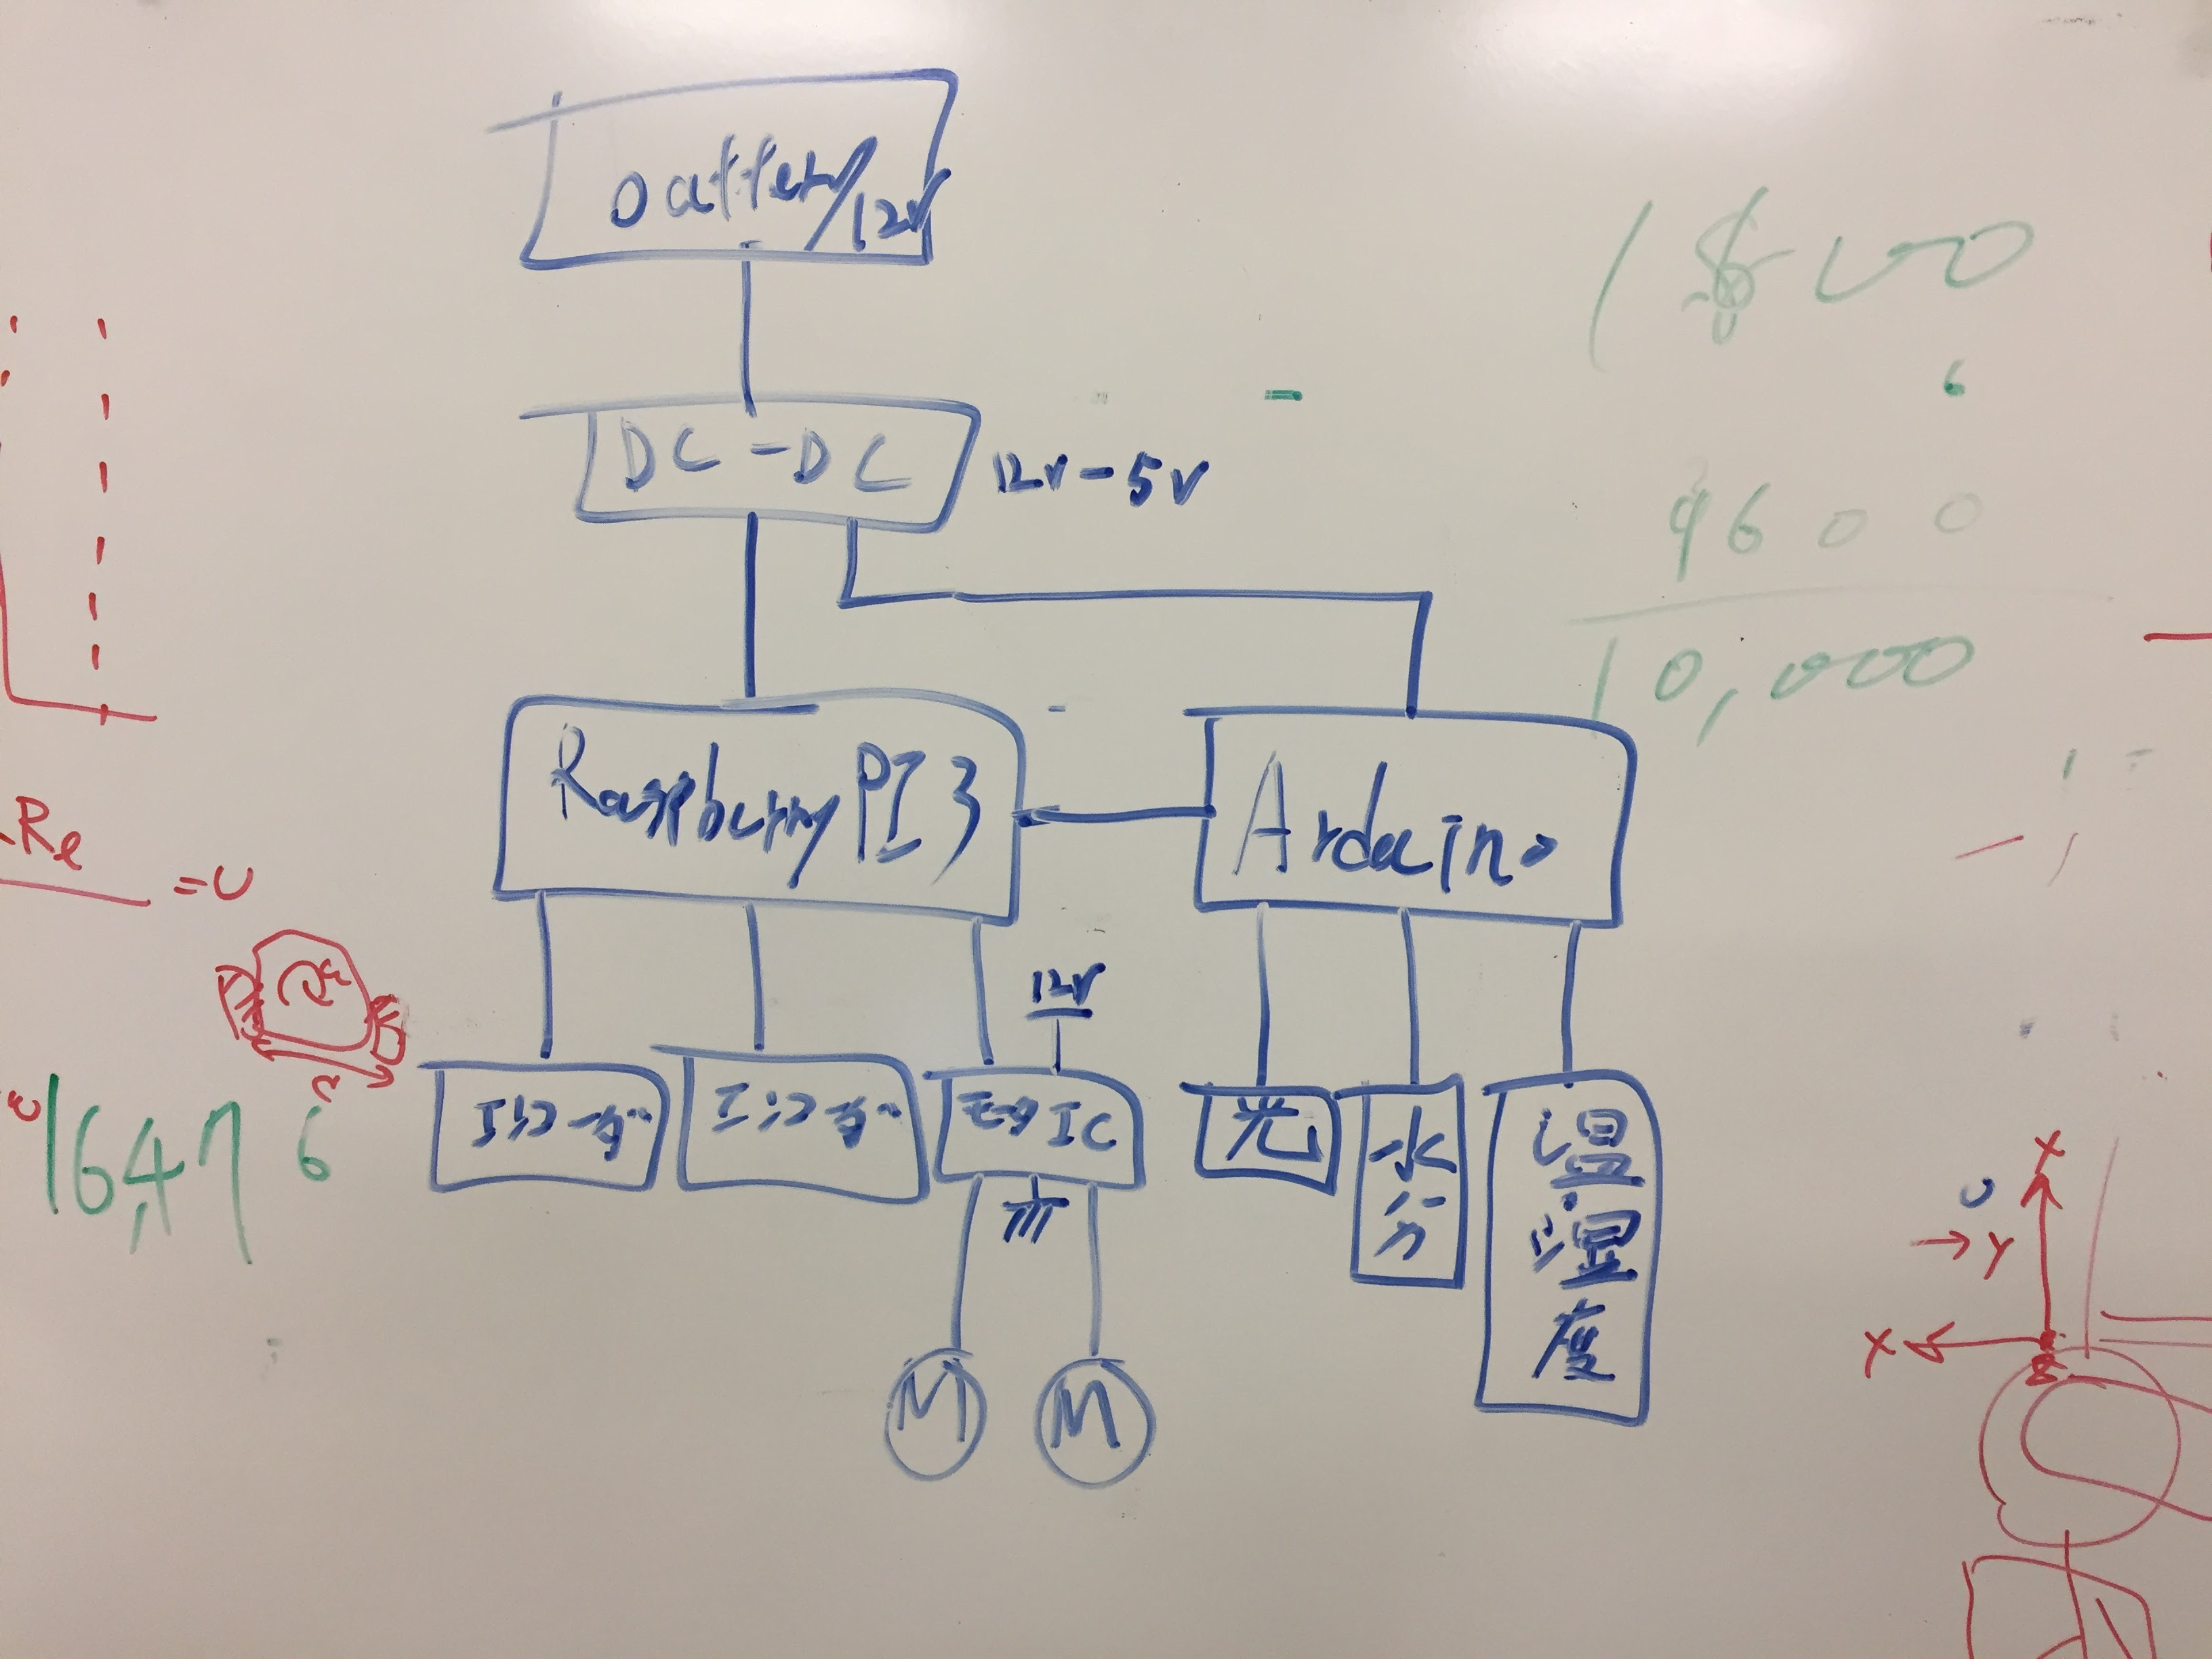
\includegraphics[width=0.4\textwidth]{img/IMG_3893.JPG}
    \caption{ロボット構成概要}
    \label{robot_hard}
\end{figure}
搭載しているコンピュタは汎用性と省スペース性に優れたRaspberry Pi 3を用いており、モータ制御とセンサ情報の管理を行っている。
同様に、アナログセンサのADコンバータには汎用性の高いArduino UNOを使用し、センサ情報はシリアル通信を用いて送信している。
搭載しているセンサは3種類で、照度、温湿度、土壌水分である。なお、照度センサは四隅に搭載し植物の影の影響を受けないようになっている。
駆動輪の取り付けは省スペース性とメンテナンス性に優れた減速ギア内蔵モータ(000?)を使用し、モータ制御ICには高効率で安価な(TA000000?)を用いている。
\subsubsection{ソフトウェア}
自律移動のためのソフトウェアの多くはRaspberry Pi上で動いており、センサで読み込んだ値を元にモータの制御を行っている。
まず、センサ情報は座標と一緒に保存され、Fig.\ref{map}ようにグリットマップで管理され、センサの種類ごとにレイヤー分けされている。
\begin{figure}[ht]
    \centering
    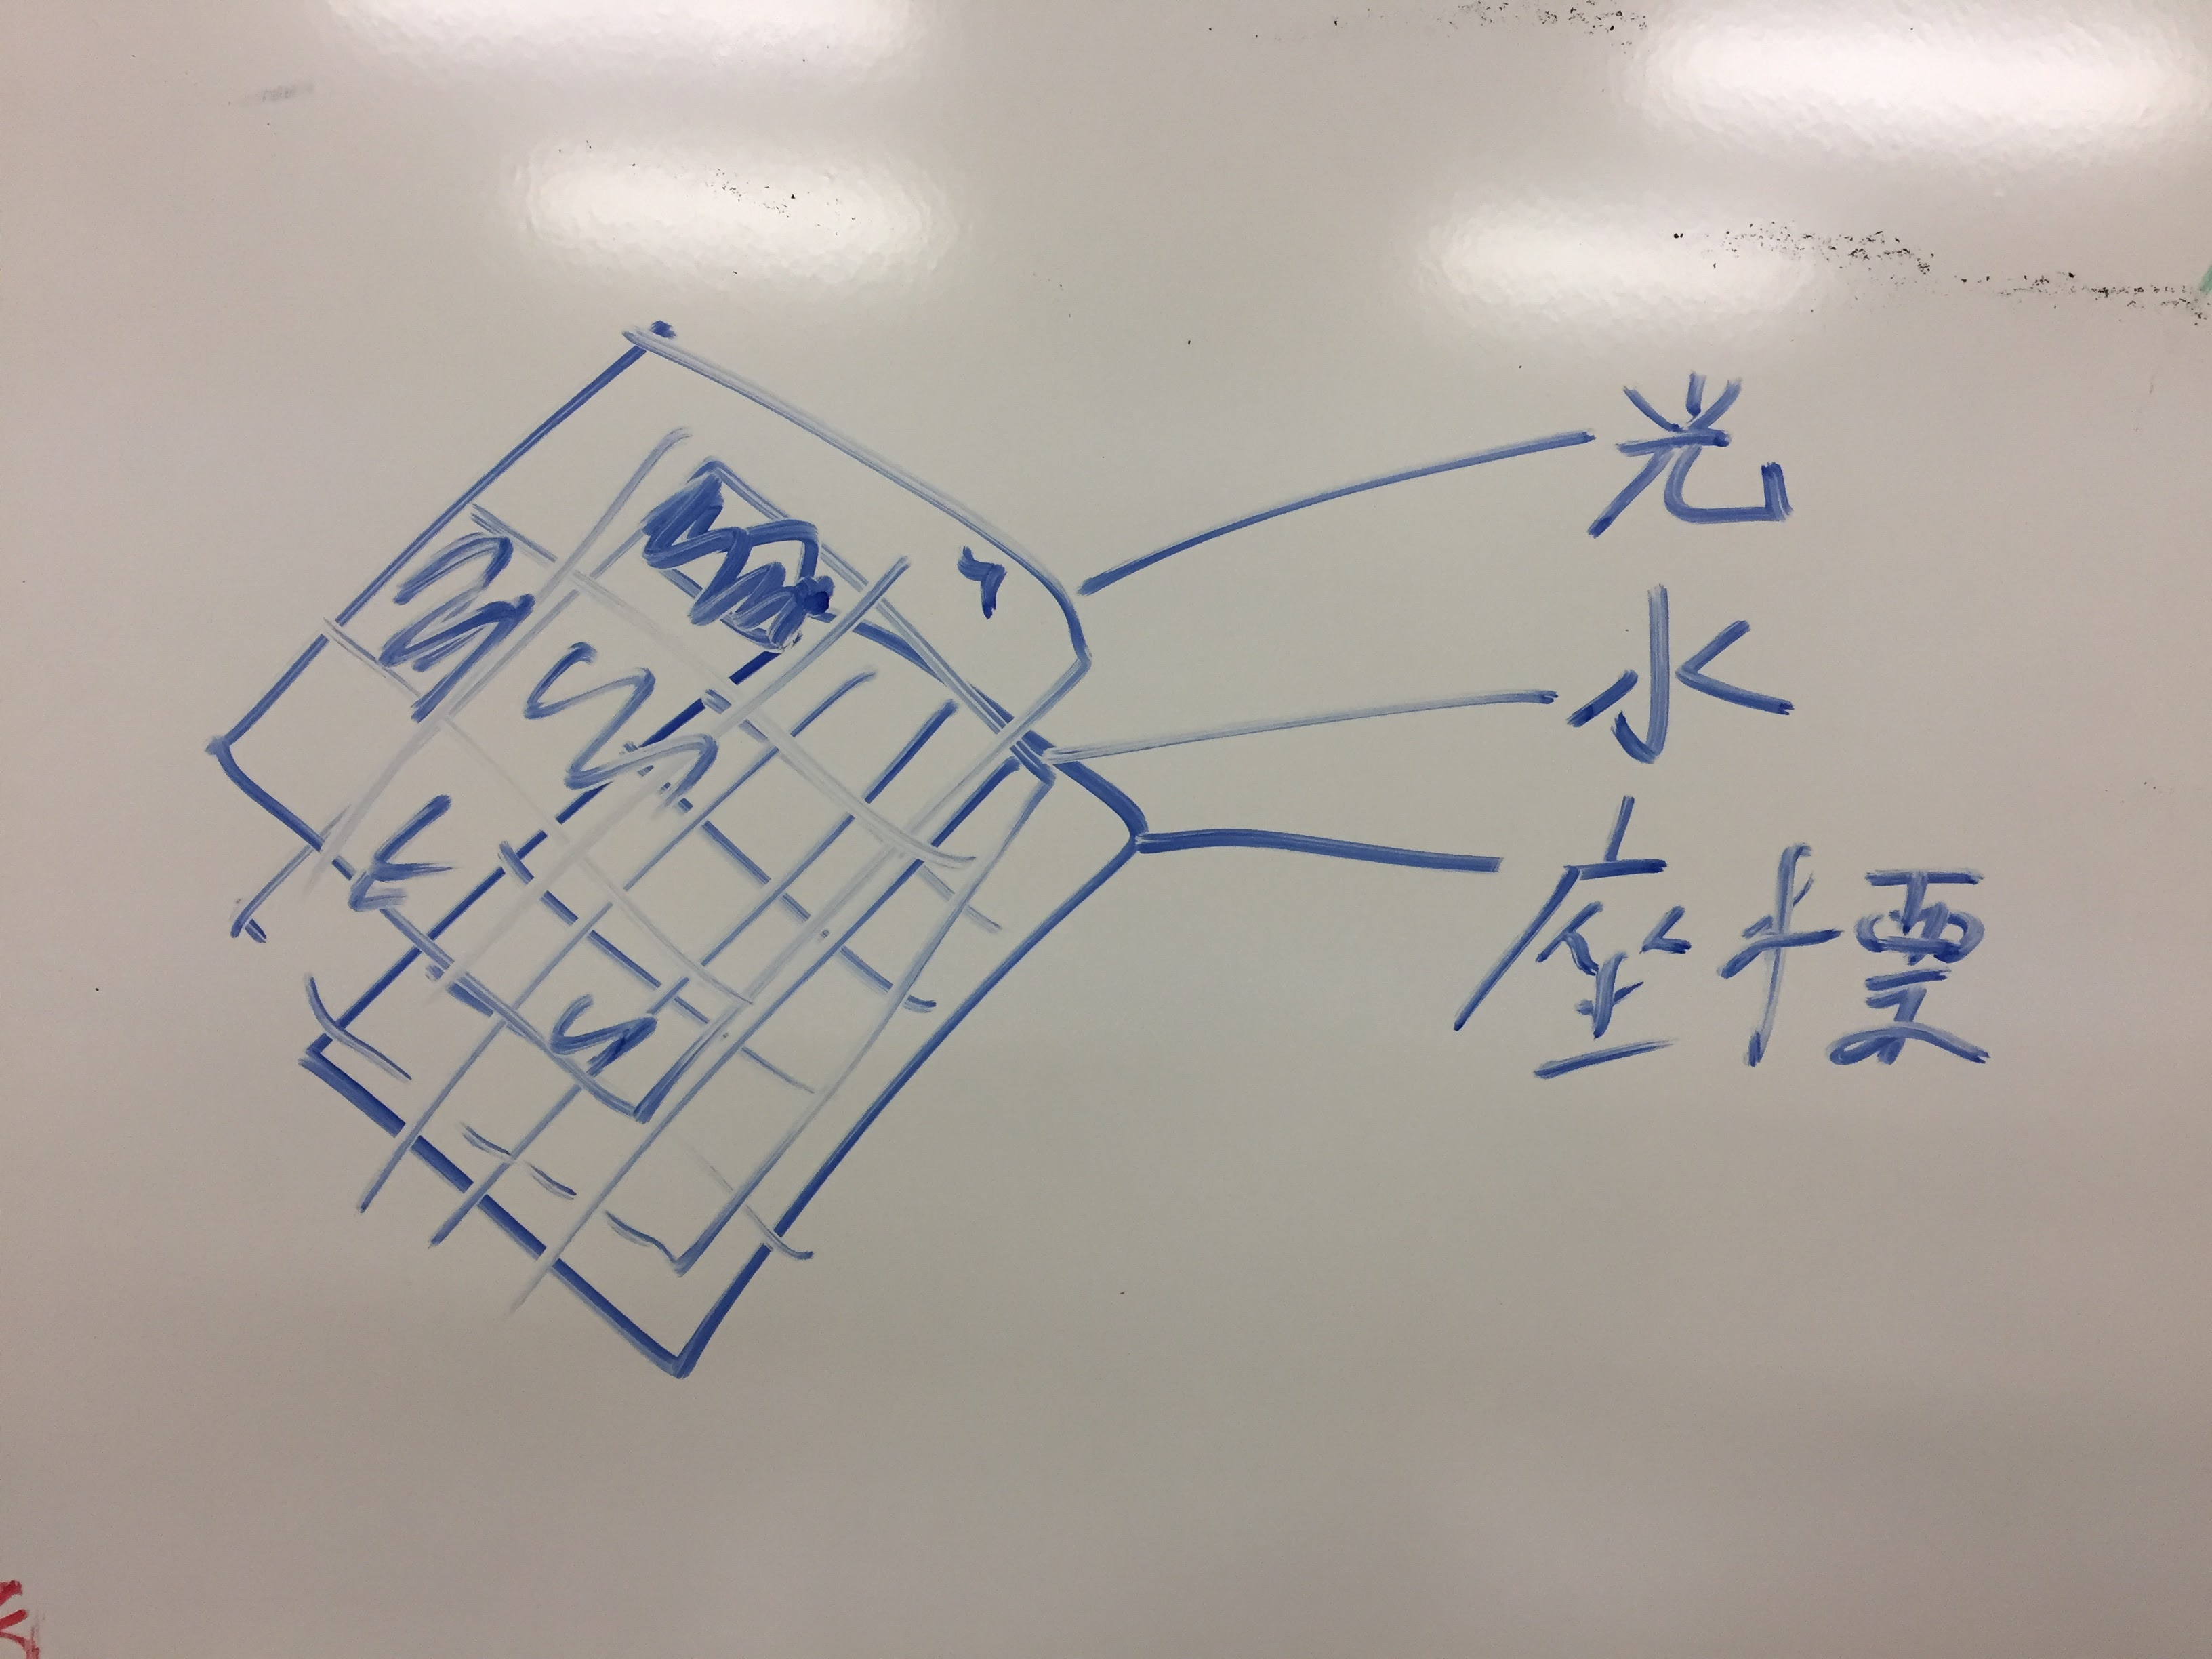
\includegraphics[width=0.4\textwidth]{img/IMG_3895.JPG}
    \caption{多次元グリットマップ}
    \label{map}
\end{figure}
この地図を元に行動計画を行う。
土壌水分量が少ない場合は次節で説明する給水ステーションに向かい、照度や温度が低い場合には周囲を散策し最適な位置に移動を行う。
そのための自律移動はモータとエンコーダの組み合わせで行っている。
安定した動きを実現するため、モータの電圧はPWM制御、速度はPID制御で運用している。
自己位置推定にはオドメトリを用いて推定している。
多少のズレはあるものの、限定空間内で行動に限れば無視できるものである。

\subsection{給水ステーション}
植物が自律的に成長するため水分の摂取は必須である。
水分を自発的に摂取するためにも、水を提供するロボットは必要なサービスである。
本ロボットは前章の自律移動ロボットとセットで利用される事を想定し製作し、距離センサを用いて近づいたものに水分を与えるものとなっている。
\subsubsection{ハードウェア}
フレームは軽く、錆びることのないアルミニウム製で、タンクは取り外しが可能となっている。
バルブの開閉機構にはRCサーボを利用し、制御のためにArduinoを用いている。
ロボットの接近を検知する距離センサは上部より下を見下ろすような形で設置し、誤検知を防いでいる。
また、ノズルの位置の調整を行うことで様々な植物に対応が可能となっている。。
\subsubsection{ソフトウェア}
ロボットの制御にはArduino UNOを使用し、サーボモータと距離センサの組み合わせで動作する。
距離センサで本ロボットの前に接近したものを検知するとRCサーボを回転させ、一定時間水分を与えた後再び再度RCサーボを回転させ戦させます。

\section{実験}
\subsection{実験方法}
本システムの評価方法として、24時間の間に人間がどれほど介入を行っているかを時間で評価する。
評価項目には水を与える時間やバッテリーを交換する時間も含める。
なお、短時間での成長ぐらいを比較することは困難を極めるため、評価項目からは除外する。
環境は冬場の室内$9m^2$とし、日の光を表現するためにスポットライトを時間ごとに動かし、温かい場所も作った実験環境Fig.\ref{experiment}で評価を行う。
\begin{figure}[ht]
    \centering
    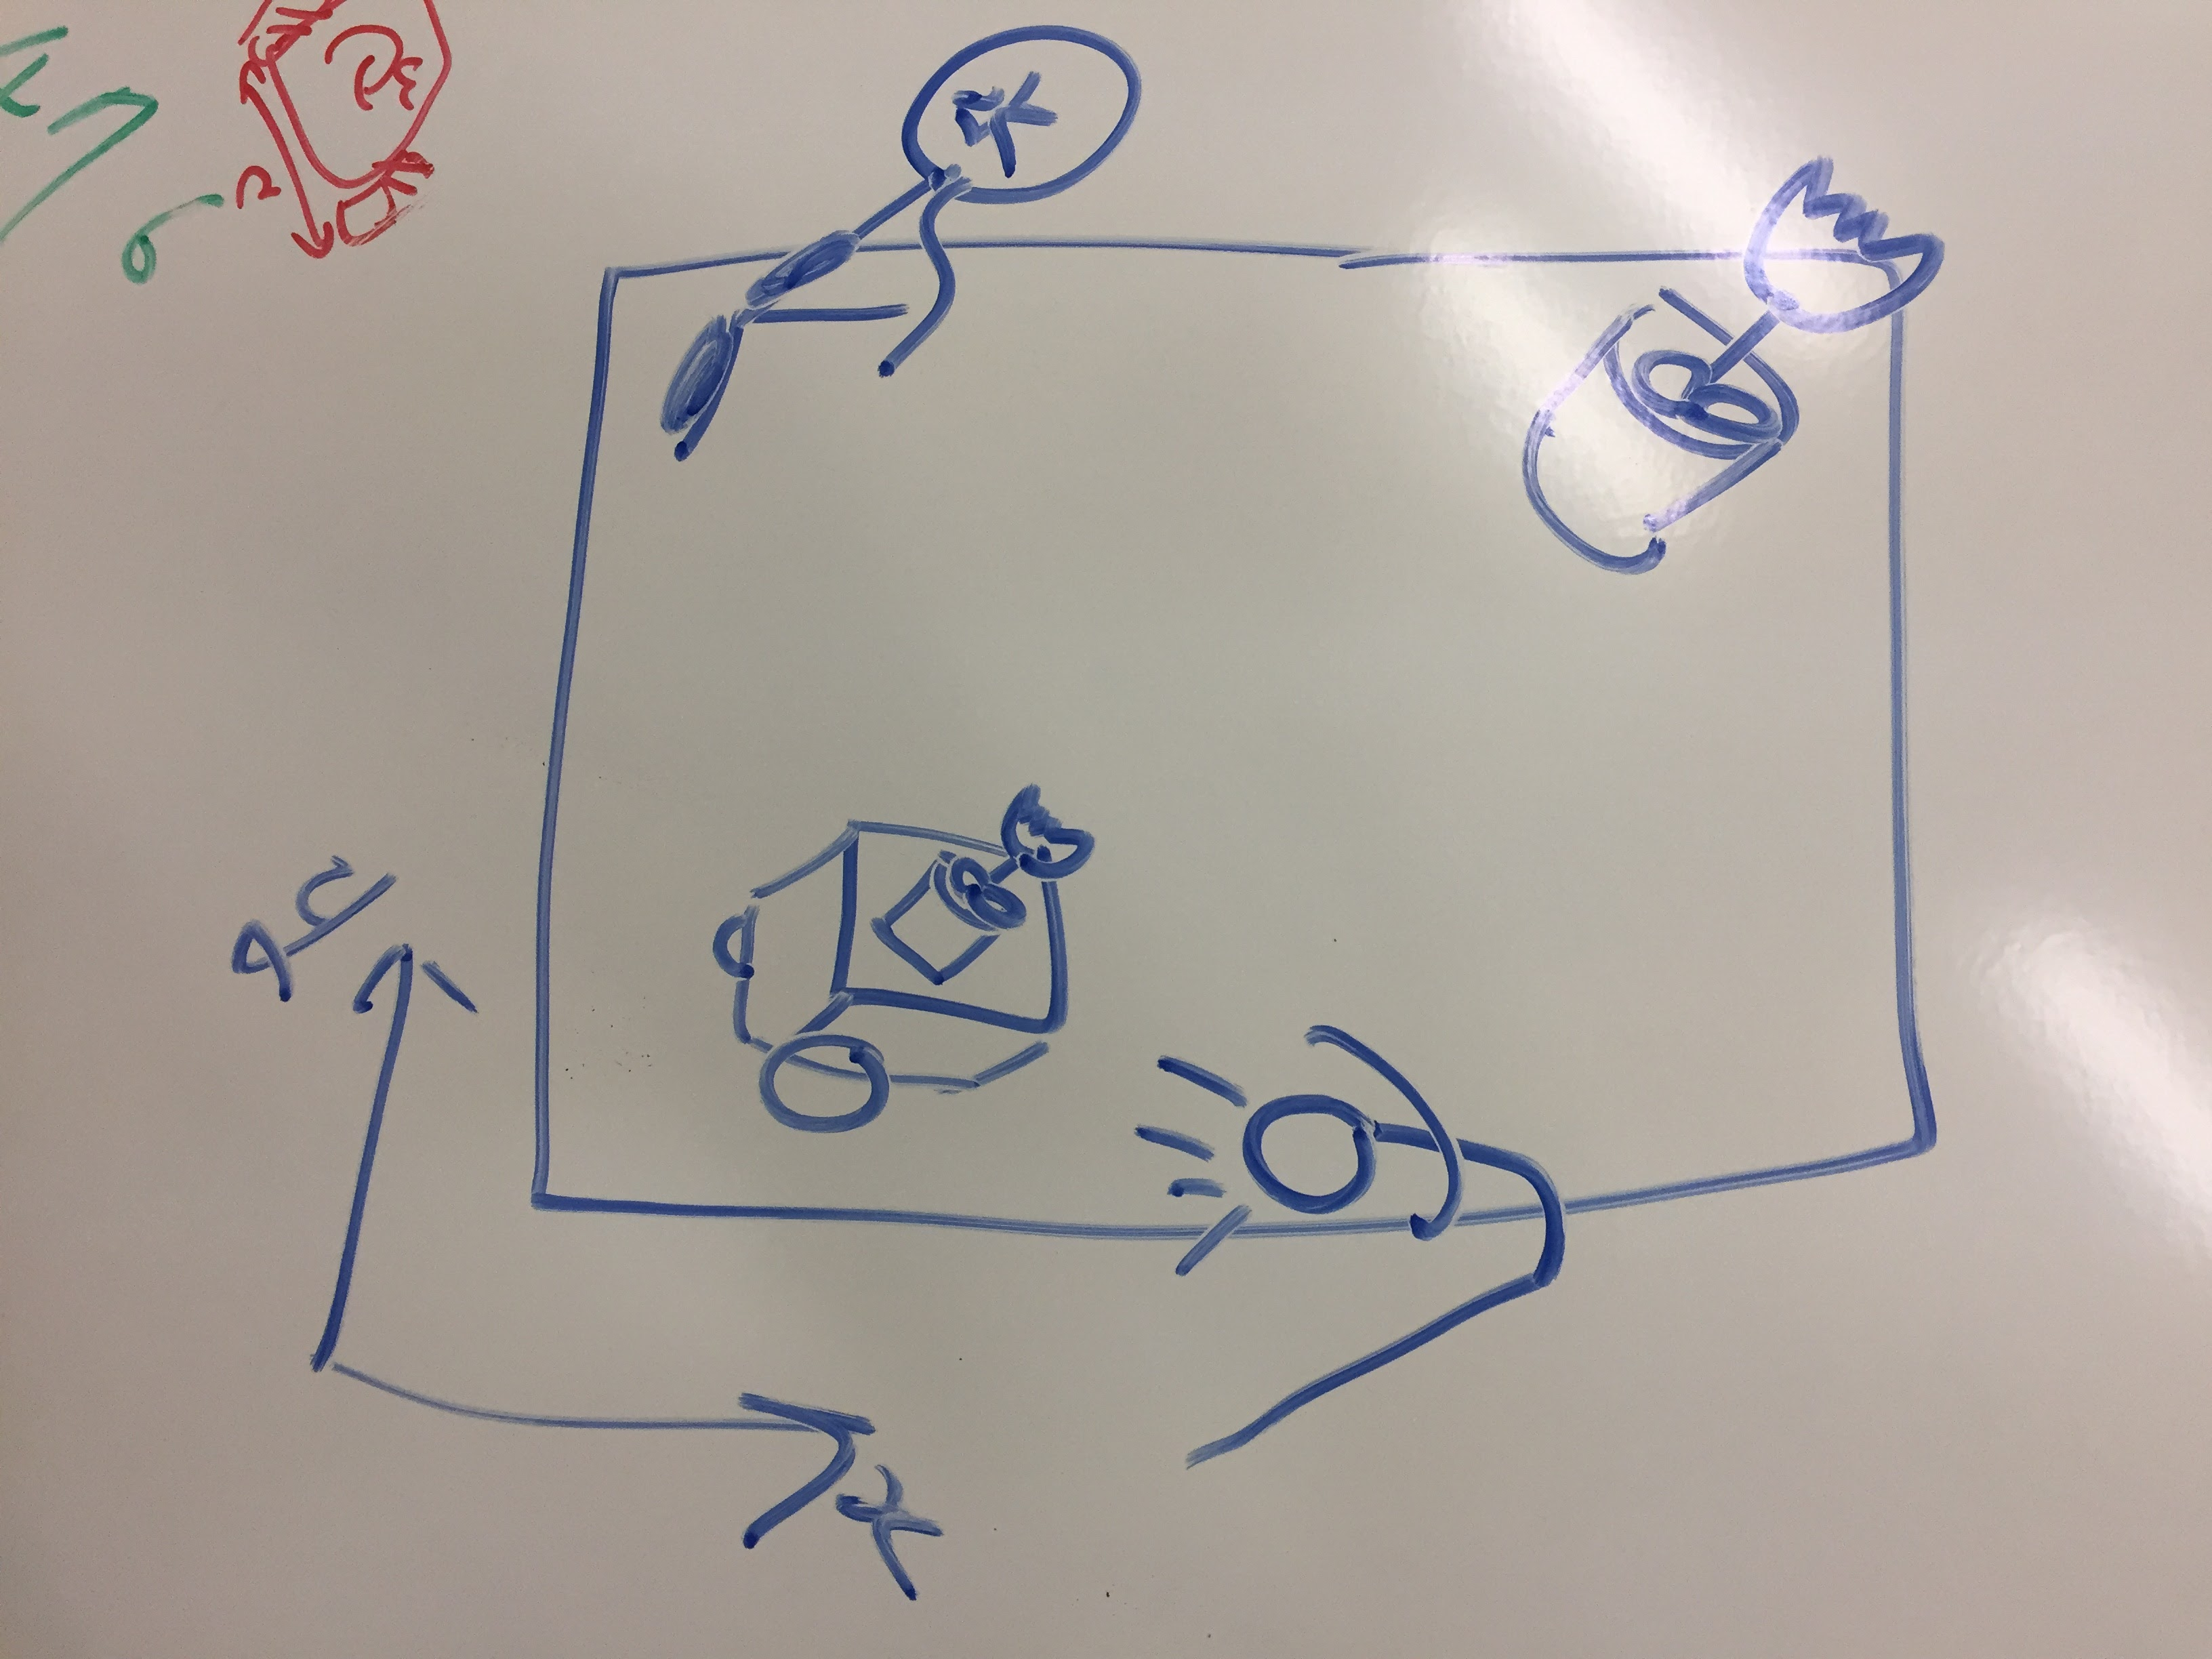
\includegraphics[width=0.4\textwidth]{img/IMG_3896.JPG}
    \caption{実験環境}
    \label{experiment}
\end{figure}
\subsection{実験結果及び考察}
人間の介在時間をまとめた実験結果はTable.\ref{hyou}に示す。
結果的にロボットのバッテリーを交換する手間がかかってしまい、本来の目的を達成できないものになった。
本来重要な評価項目である成長具合を確認できず、期間が長ければ異なる結果を示す可能性もある。
\begin{table}[ht]
    \centering
    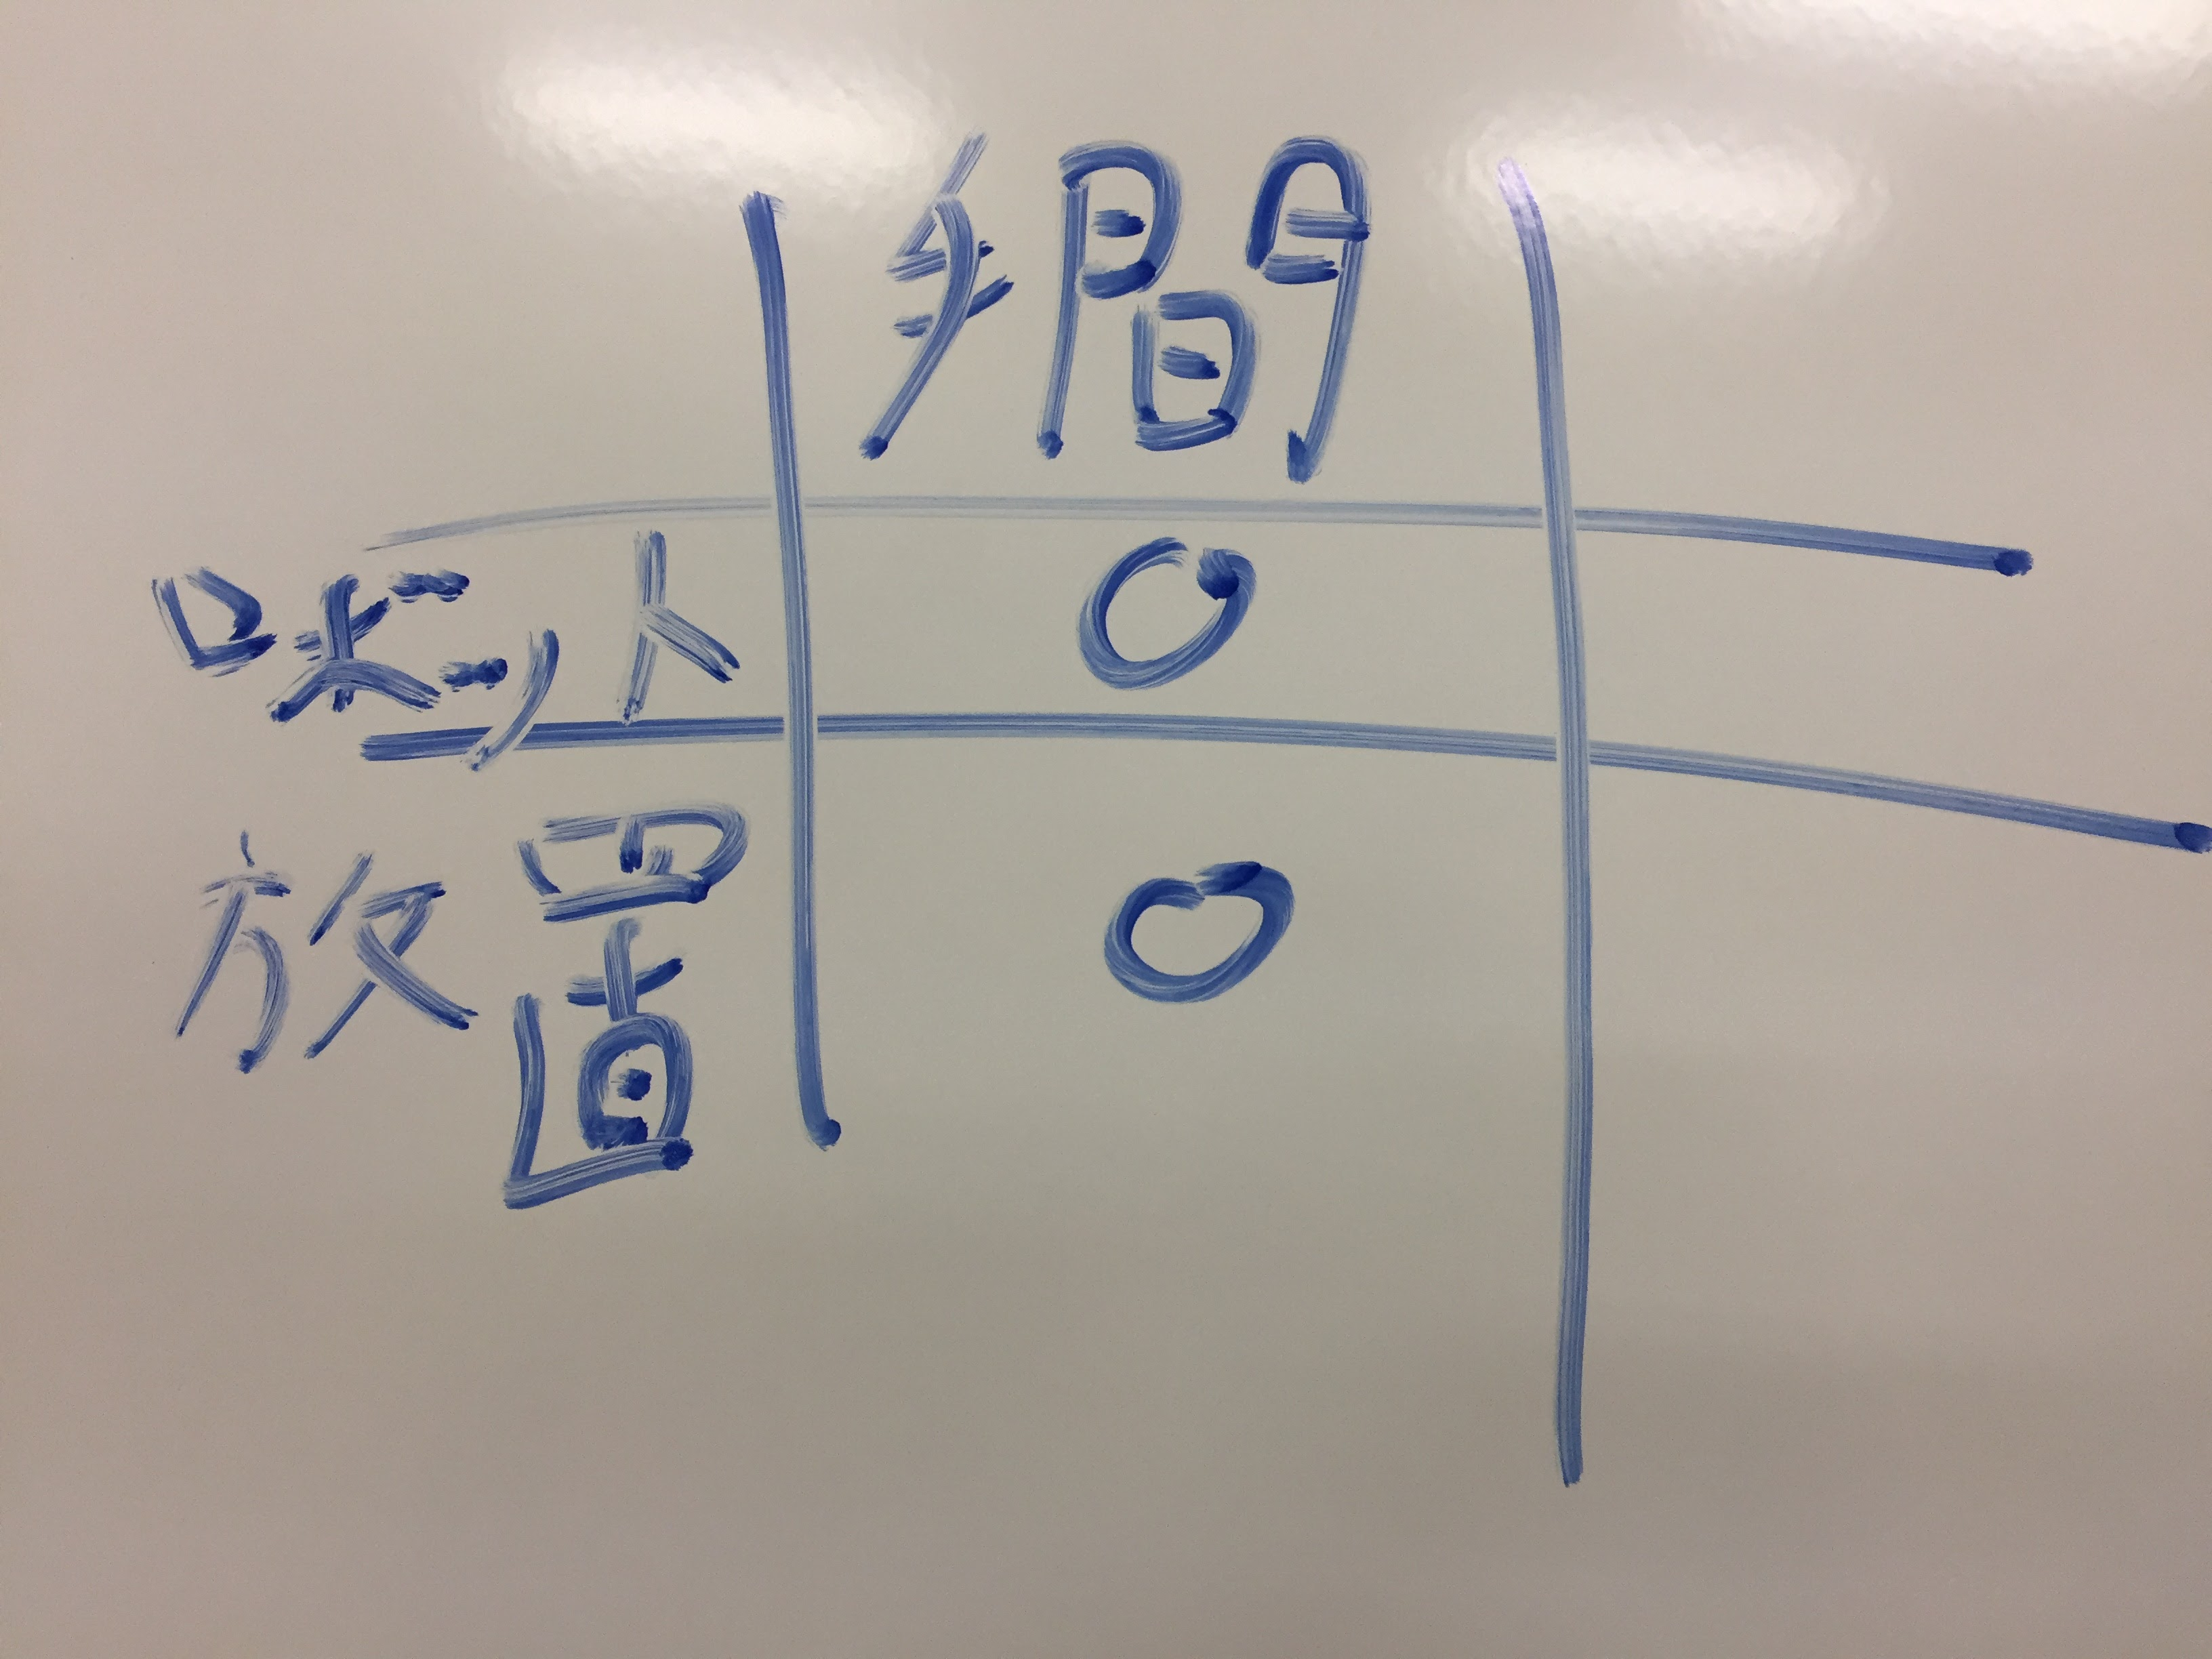
\includegraphics[width=0.4\textwidth]{img/IMG_3897.JPG}
    \caption{人間の介在時間}
    \label{hyou}
\end{table}
\section{おわりに}
ここも後ほど書きます。

\begin{thebibliography}{10}

%%参考文献
\bibitem{Paper01}
東海太郎, 東海二郎: XXXに基づくロボットのシステム制御の開発,
日本ロボット学会誌,{\bf xx}-xx, pp.xxx-xxx (20xx)

\end{thebibliography}

\end{document}
